% \newcommand{\prototitle}{Versuch 2 - Statistik}
% \newcommand{\Fachbereich}{Praktikum Messtechnik}
% \input{../packages/tu_header}

\newcommand{\institut}{Institut f\"ur Telekommunikationssysteme}
\newcommand{\fachgebiet}{Nachrichten\"ubertragung}
\newcommand{\veranstaltung}{Praktikum Nachrichten\"ubertragung}
\newcommand{\pdfautor}{\"Ozg\"u Dogan (326 048), Boris Henckell (325 779)}
\newcommand{\autor}{\"Ozg\"u Dogan (326 048)\\ Boris Henckell (325 779)}
\newcommand{\gruppe}{Gruppe: }
%\newcommand{\betreuer}{Betreuer: Mahmoud Felk}


\newcommand{\pdftitle}{Nachrichten\"ubertragung\ Praktikum\ 01}
\newcommand{\prototitle}{Praktikum 01 \\ Einf\"uhrung in MATLAB}


\input{../../packages/tu_header_8}

%---------------------------------------------------------------------
%---------------------------------------------------------------------
%---------------------------------------------------------------------
\section{Einleitung}




\section{Vorbereitungsaufgaben}

    \begin{quote}
    Die Vorbereitungsaufgabe lautet, die Varianz von gleichverteiltem weißen Rauschen $N$ mit der
    Verteilungsdichtefunktion $p_{N(n)} = \frac{1}{2A} \sqcap_{2A} (n)$ zu berechnen.\\
    Zuerst berechnen wir den Mittelwert $\mu$:
   	\begin{equation*}
    	\begin{split}
    		\mu &= \int_{-\infty}^{+\infty} n \frac{1}{2A} \sqcap_{2A} (n) \mathrm dn\\
    		&= \int_{-A}^{+A} n \frac{1}{2A} \mathrm dn\\
    		&= \left[ \frac{1}{2A} \frac{1}{2} n^2 \right]_{-A}^{+A}\\
    		&= \frac{1}{4A} (A^2-(-A)^2)\\
    		&= 0
    	\end{split}
    \end{equation*}
    
    Dannach berechnen wir die Leistung des Signals$P$:\\
    \begin{equation*}
    	\begin{split}
    		P &= \int_{-\infty}^{+\infty} n^2 \frac{1}{2A} \sqcap_{2A} (n) \mathrm dn\\
    		&= \int_{-A}^{+A} n^2 \frac{1}{2A} \mathrm dn\\
    		&= \left[ \frac{1}{2A} \frac{1}{3} n^3 \right]_{-A}^{+A}\\
    		&= \frac{1}{6A} (A^3-(-A)^3)\\
            &= \frac{2A^3}{6A} = \frac{1}{3} A^2\\
    	\end{split}
    \end{equation*}
    
    Mit diesen Werten läßt sich die Varianz wie folgt berechnen:
    \begin{equation*}
    	\begin{split}
    		\sigma^2 &= P - \mu^2\\
    		&= \frac{1}{3} A^2 - 0 = \frac{1}{3} A^2
    	\end{split}
    \end{equation*}
	\end{quote}
         	


%--------------------------------------------------------------------
%--------------------------------------------------------------------            
\section{Praktische Aufgaben}
\begin{quote}
    \subsection{Simulation eines Zufallsexperiments in Matlab}
    \begin{quote}
        Im ersten Teil des Labortermins haben wir uns mit der Simulation eines Zufallsexperiments beschäftigt. Dazu
        haben wir die Vorgegebene Datei Aufgabe1.m stückweise erweitert. In der Ursprungsversion simuliert Aufgabe1.m
        ein Zufgallsereigniss mit 10000 Würfen eines Würfels und plottet anschließend das Histogramm dieser
        Simulation.\\
        
        \subsubsection{10000 facher  Wurf eines Würfels}
		\begin{quote}
        Im ersten Teil haben wir die Datei so ergänzt, dass die Wahrscheinlichkeitsverteilungsdichtefunktion von diesem
        Zufallsereigniss dargestllt wurde. Dazu haben wir die Anzahl der Treffer durch die Anzahl der Würfe geteilt
        und das Ergebiss plotten lassen. Da es sich um einen fairen Würfel handelt erwarten wir eine gleichmäßig
        verteilte Verteilungsdichtefunktion.
            \begin{figure}[H]
            \centering
                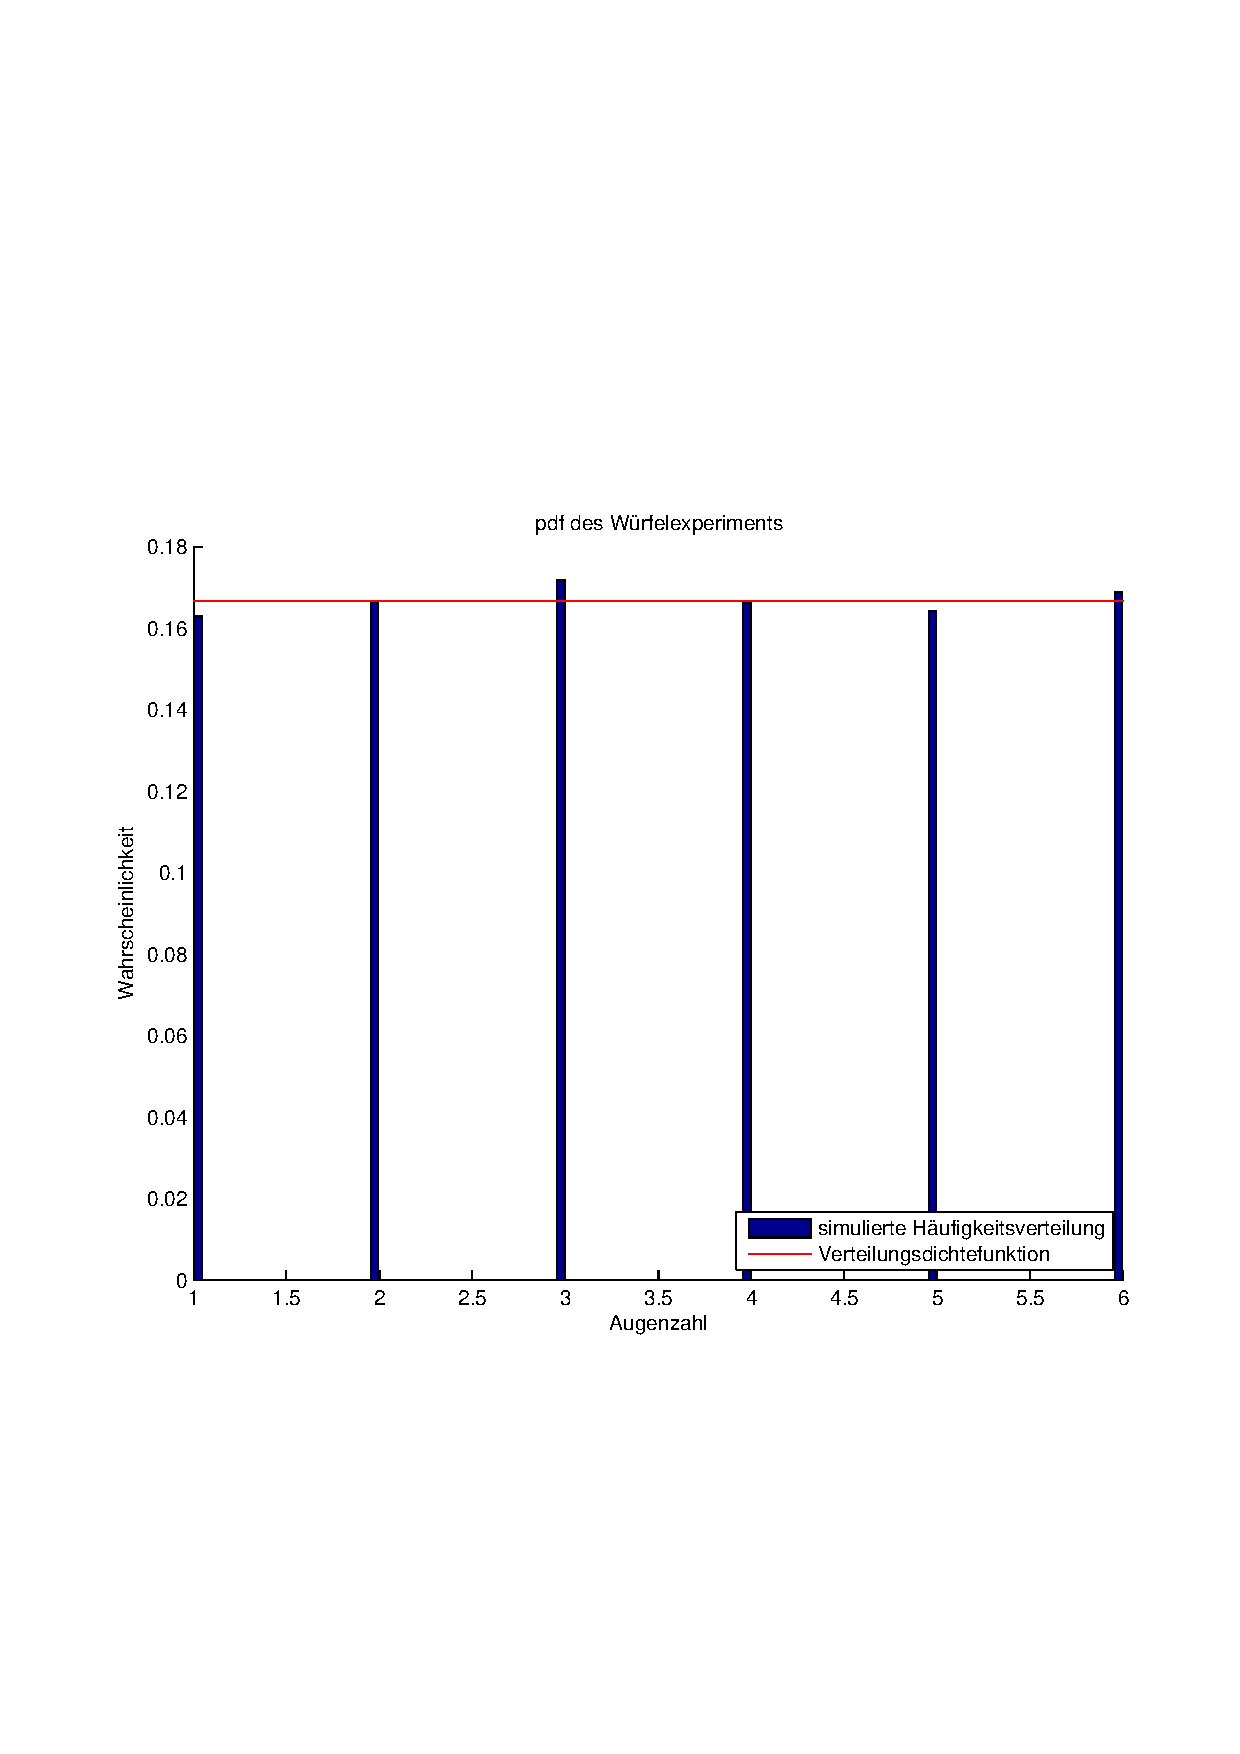
\includegraphics[scale=0.7, trim = 0cm 0cm 0cm 0cm, clip]{./Bilder/1wuerfelpdf}
                    \caption{Verteilungsdichtefunktion 1 Würfel 10000 Würfe}
                    \label{fig:./Bilder/1wuerfelpdf}
            \end{figure}
    
		\end{quote}
        
        \subsubsection{10000 facher Wurf zweier Würfel}
		\begin{quote}
			Im zweiten Teil haben wir die Simulation soweit verändert, dass bei jedem Wurf zwei Würfel simmuliert wurden deren
			Augenzahl aufsummiert wurden. Damit auch der zweite Würfel unabhängig simuliert wird haben wir einen zweiten Vektor
			erstellt mit einem zufälligen $10000$-fachen Würfelereigniss und die beiden Vektoren addiert. In hinblick auf die
			folgende Aufgabe, bei der wesentlich mehr Würfel pro wurf addiert werden sollten, wurde uns aber auch beigebracht,
			dass die rand-funktion schon eine Lösung für dieses Problem integriert hat. Und desshalb haben wir anstatt des
			zweiten Vektors einfach den zweiten Parameter der rand-funktion auf zwei gestellt und somit unabhängige Würfel
			simuliert.\\
			Auch von diesem Experiment haben wir die Verteilungsdichtefunktion errechnet und plotten lassen.\\
			Da sich die Verteilungsdichtefunktion von zwei statistisch unabhängigen Erignissen auch als Faltung der einzelnen
			Verteilungsdichtefunktinen darstellen lassen kann erwarten wir in diesem Fall eine Dreieckförmige
			Verteilungsdichtefunktion.
		\end{quote}
        
        \subsubsection{10000 facher Wurf meherer Würfel}
		\begin{quote}
			Um den zentralen Grenzwertsatz der Statistik nachzuvollziehen erhöhen wir schrittweise die Anzahl der Würfel, die
			miteinander addiert werden, und erstellen deren Verteilungsdichtefunktionen. Laut Grenzwertsatz erwarten wir, dass
			sich die resultierende Verteilungsdichtefunktion sich an eine Gaußverteilung anpasst.
		\end{quote}
		
		\subsubsection{Verteilungsdichtefunktionen der einzelnen Versuche}
		\begin{quote}
			    \subsection{Ergebnisse Vorbereitungsaufgaben}
    \begin{quote}
                                %4 Grafiken:
            \begin{center}
            \begin{tabular}{ll}

            \hspace{-4em}
                \begin{minipage}{0.6\textwidth}

                    \begin{figure}[H]
                        \label{fig:}
                        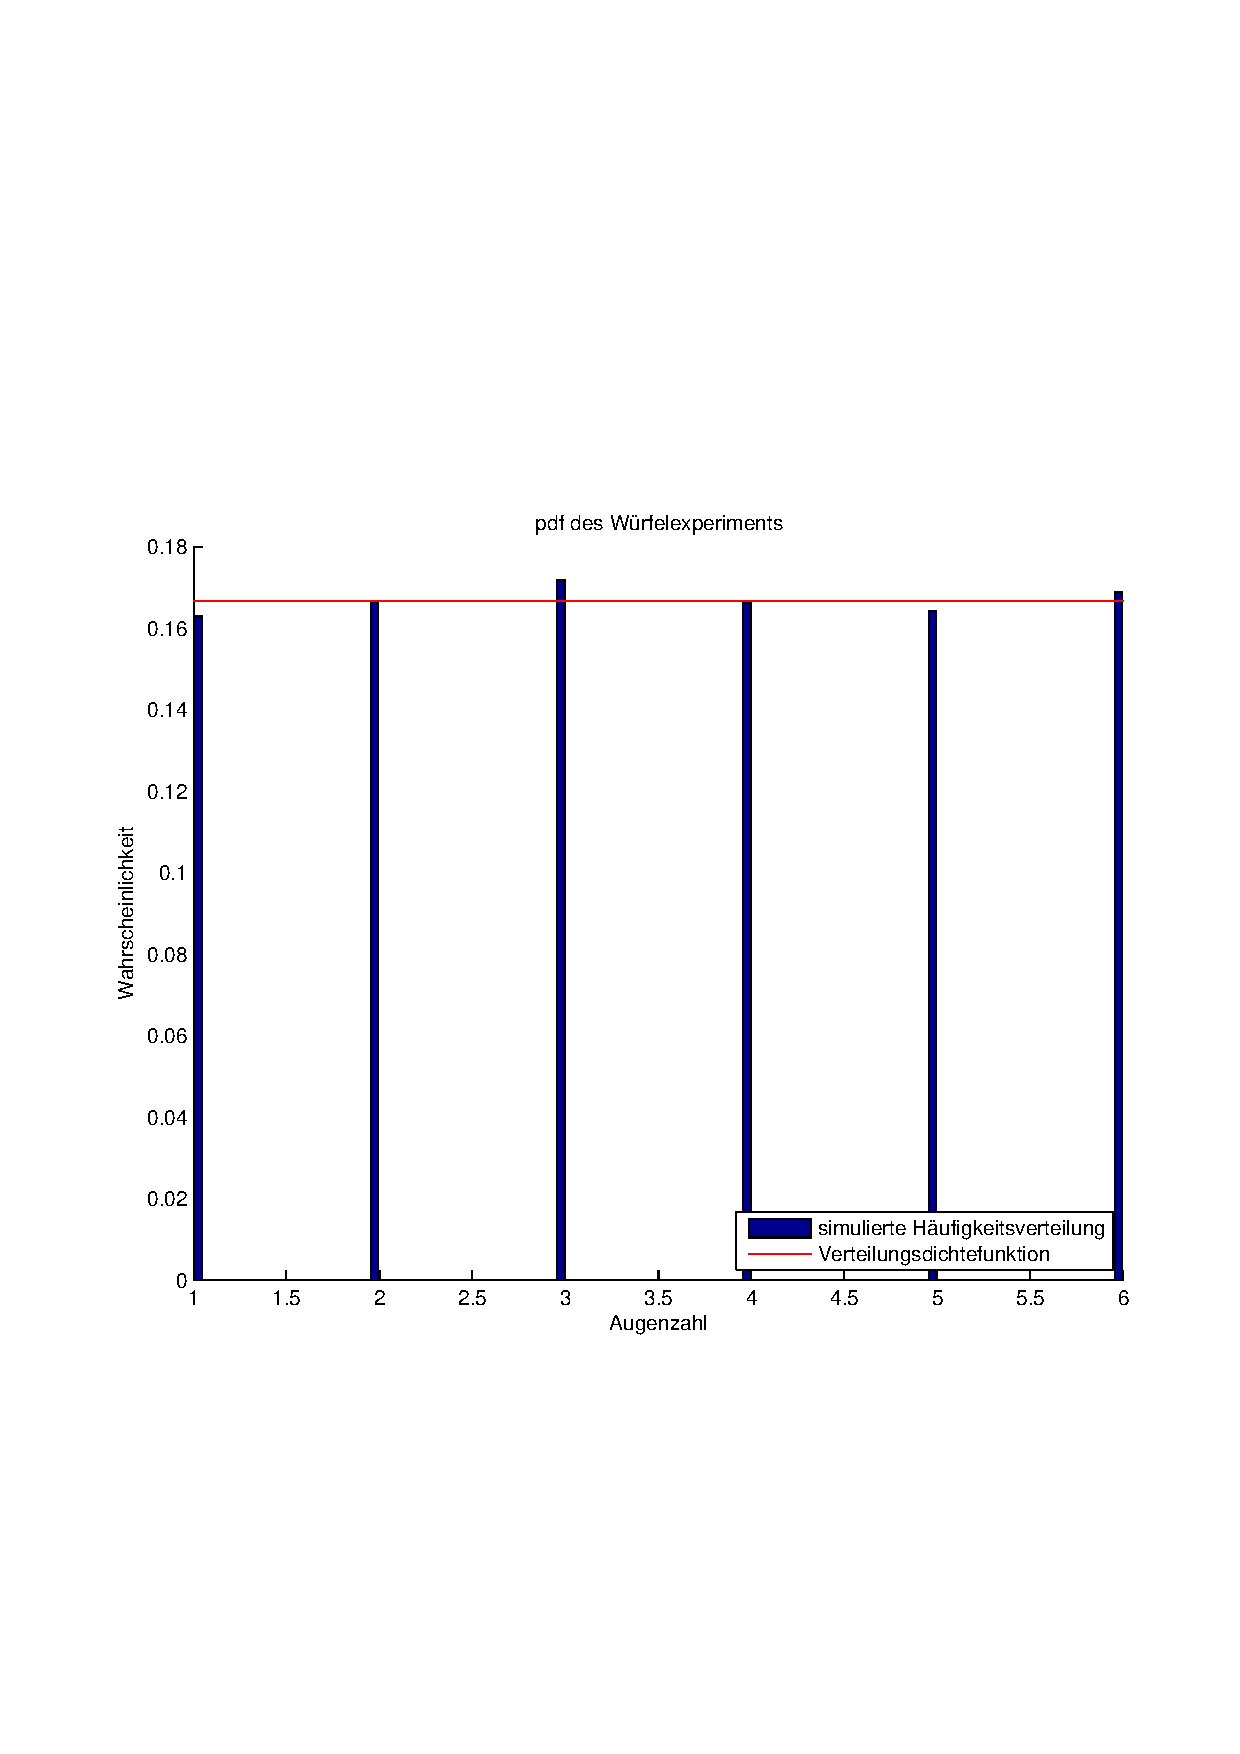
\includegraphics[scale=0.3]{./Bilder/1wuerfelpdf} %FIXME [width=640px,
                         %height=474px]
                        \caption{Verteilungsdichtefunktion 1 Würfel 10000 Würfe}
                    \end{figure}

                \end{minipage}
                \begin{minipage}{0.6\textwidth}

                    \begin{figure}[H]
                        \label{fig:}
                        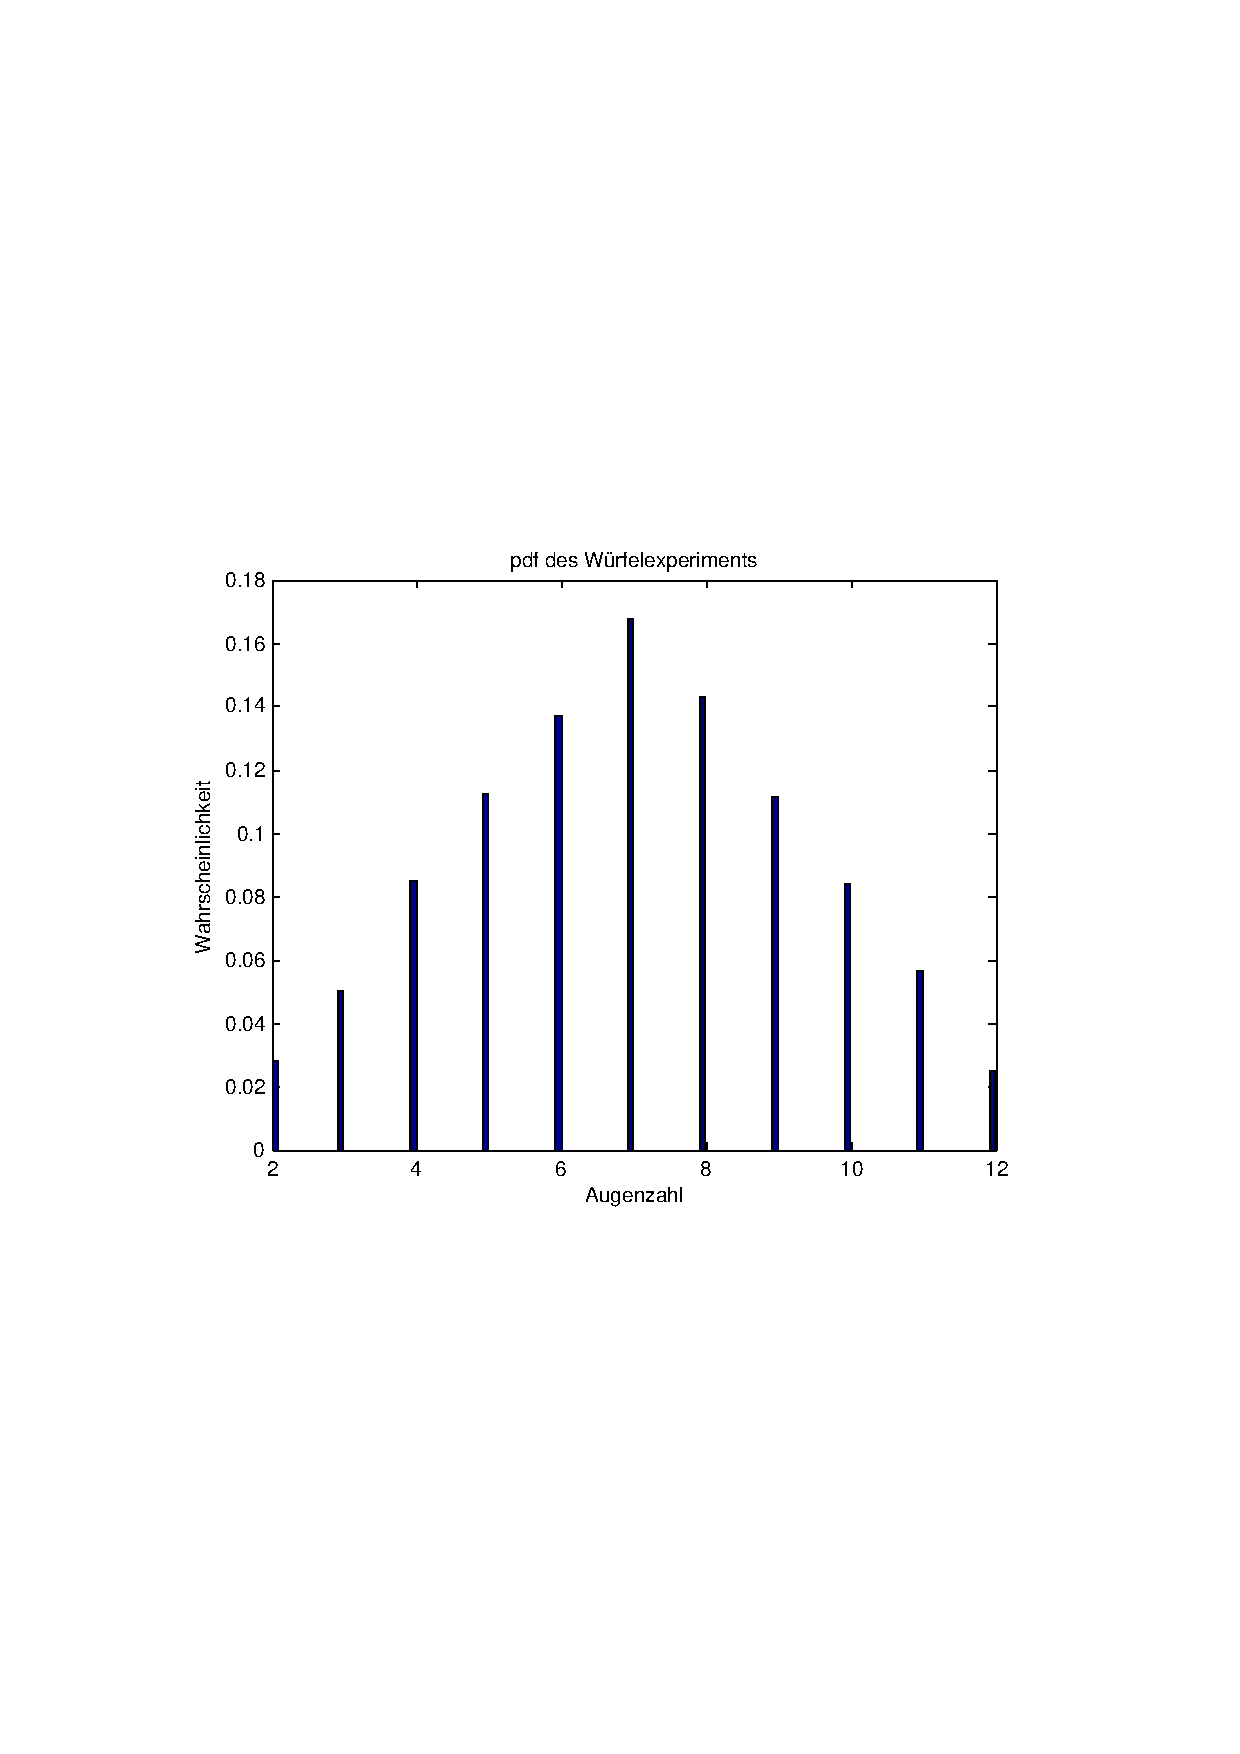
\includegraphics[scale=0.3]{./Bilder/2wuerfelpdf} %FIXME [width=640px,
                         %height=474px]
                        \caption{Verteilungsdichtefunktion 2 Würfel 10000 Würfe}
                    \end{figure}
                \vspace{-1.5em}

                \end{minipage}

            \end{tabular}
            \end{center}

                        %4 Grafiken:
            \begin{center}
            \begin{tabular}{ll}

            \hspace{-4em}
                \begin{minipage}{0.6\textwidth}

                    \begin{figure}[H]
                        \label{fig:}
                        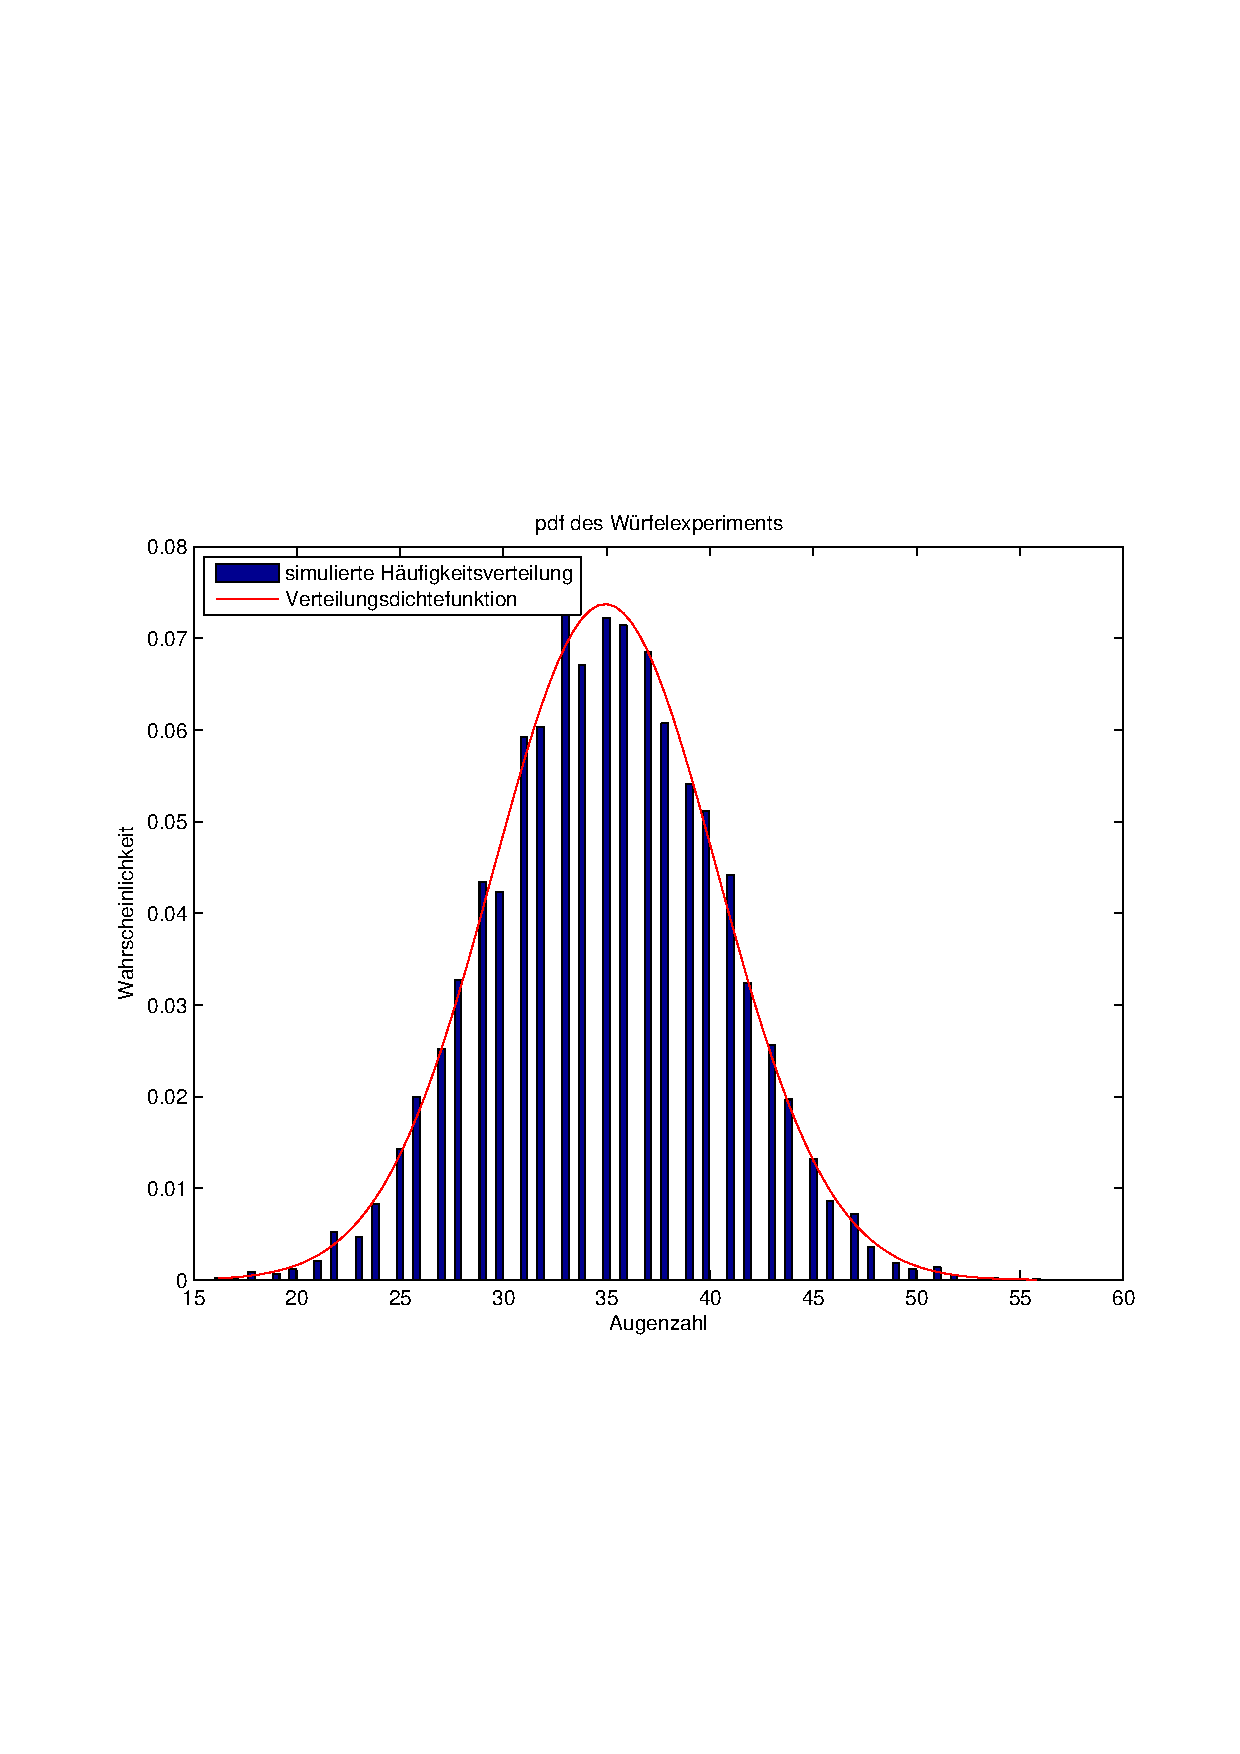
\includegraphics[scale=0.3]{./Bilder/10wuerfelpdf} %FIXME [width=640px,
                        % height=474px]
                        \caption{Verteilungsdichtefunktion 10 Würfel 10000 Würfe}
                    \end{figure}

                \end{minipage}
                \begin{minipage}{0.6\textwidth}

                     \begin{figure}[H]
                        \label{fig:}
                        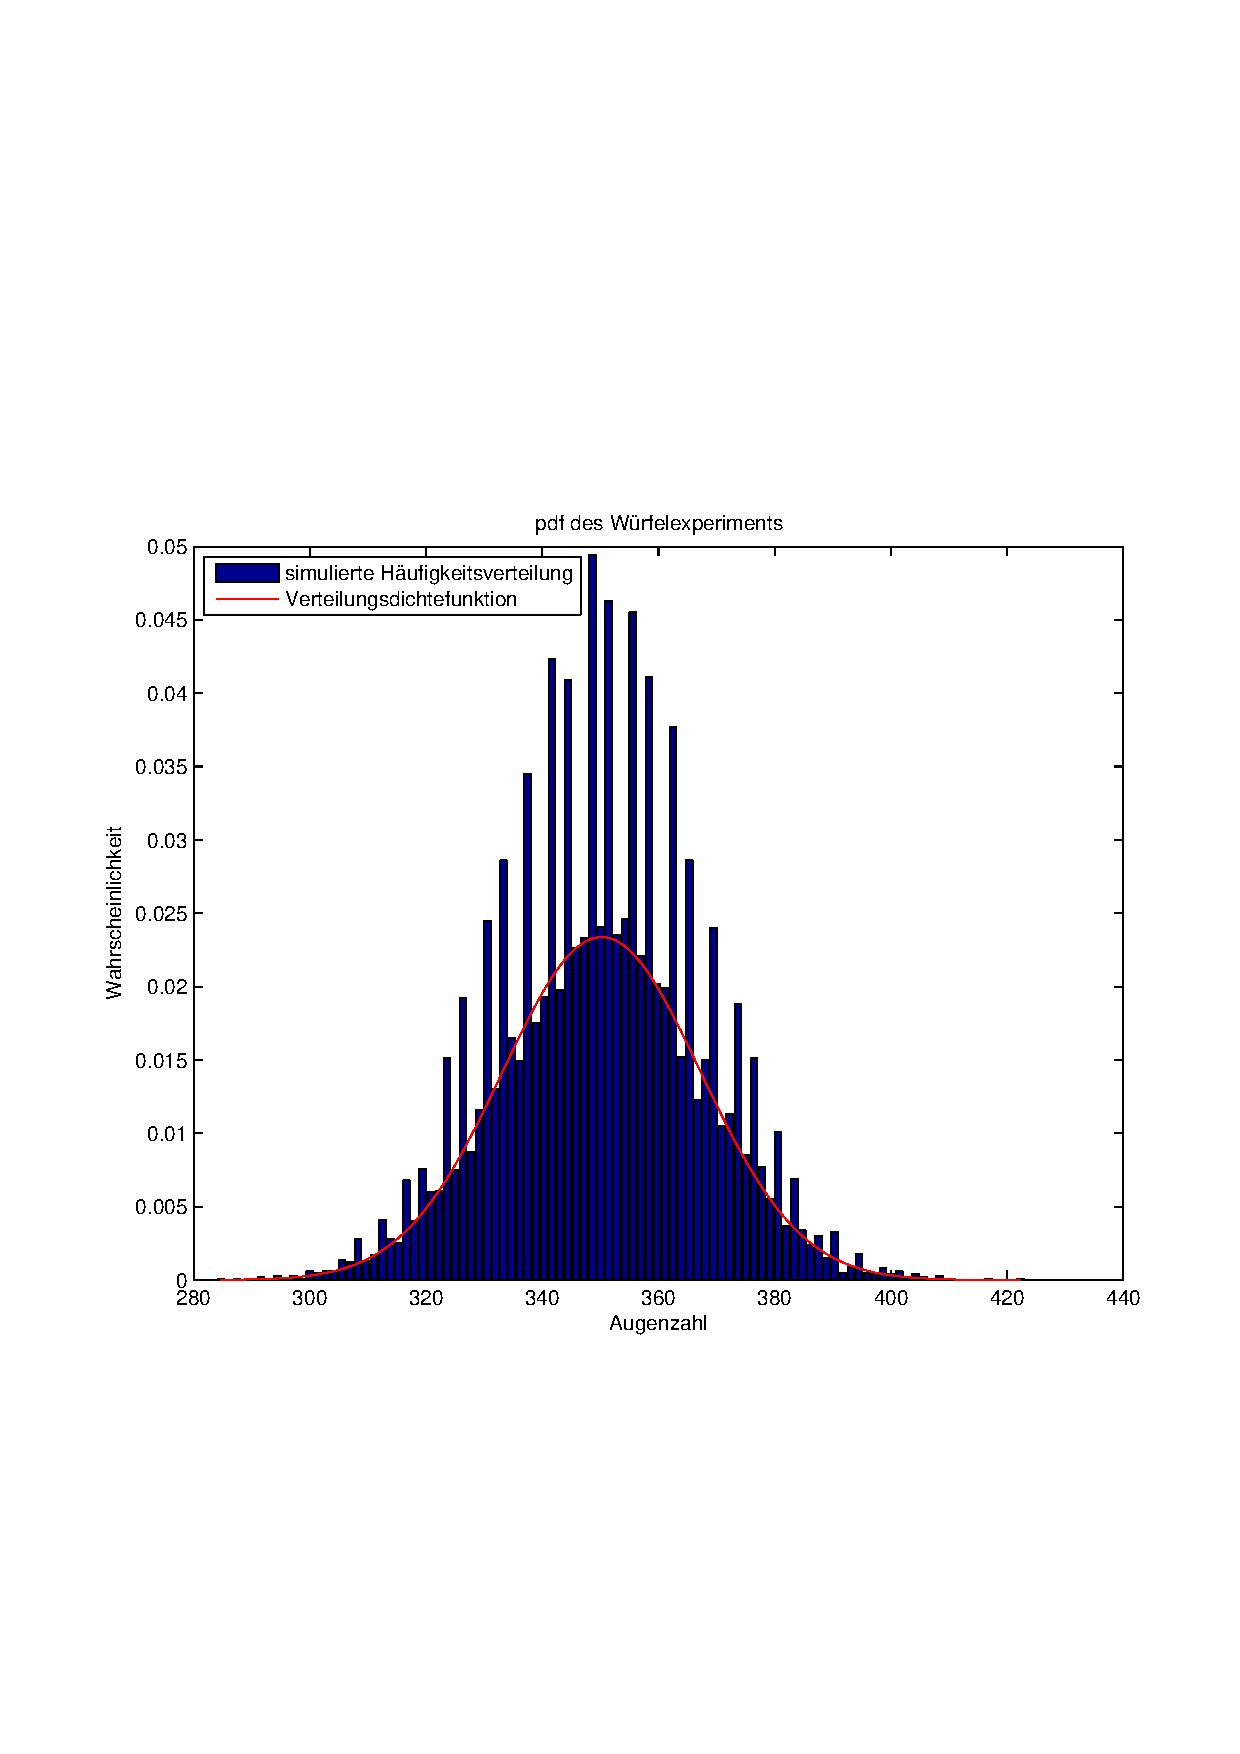
\includegraphics[scale=0.3]{./Bilder/100wuerfelpdf} %FIXME [width=640px,
                        % height=474px]
                        \caption{Verteilungsdichtefunktion 100 Würfel 10000 Würfe}
                    \end{figure}
               \vspace{-1.5em}

                \end{minipage}

            \end{tabular}
            \end{center}

                        %4 Grafiken:
            \begin{center}
            \begin{tabular}{ll}

            \hspace{-4em}
                \begin{minipage}{0.6\textwidth}

                    \begin{figure}[H]
                        \label{fig:}
                        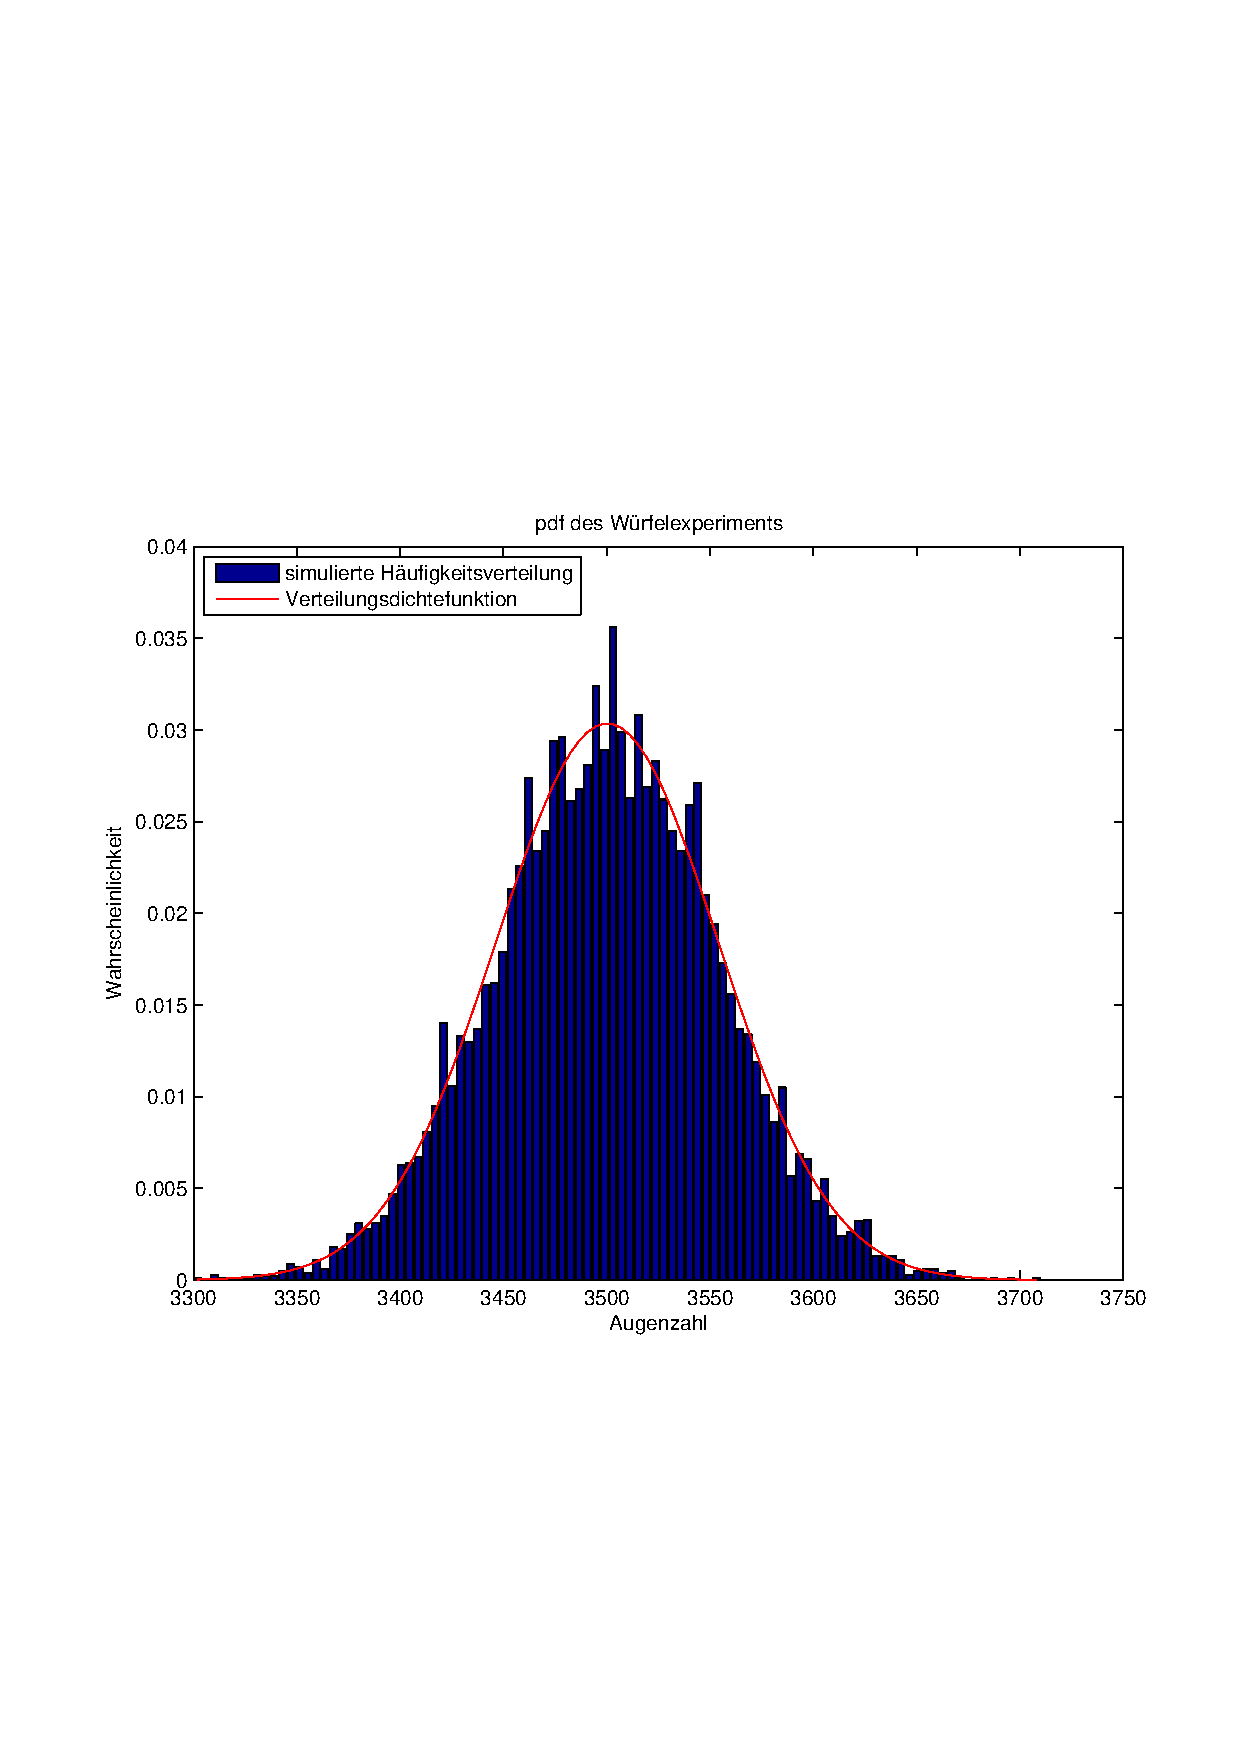
\includegraphics[scale=0.3]{./Bilder/1000wuerfelpdf} %FIXME [width=640px,
                        % height=474px]
                        \caption{Verteilungsdichtefunktion 1000 Würfel 10000 Würfe}
                    \end{figure}

                \end{minipage}

            \end{tabular}
            \end{center}
		
		\end{quote}
    \end{quote}	
    \subsection{Rauschbehafteter Übertagungskanal}
    \begin{quote}
        Im nächsten Abschnitt haben wir uns mit einem Rauschbehafteten Übertragungskanal beschäftigt. Hierfür haben wir
        an dem Telecommunications Trainer ein Pseudozufälliges Signal erzeugt und additiv Rauschen hinzugefügt(beim
        ersten Durchgang $-20dB$, beim zweiten $-6dB$ und beim letzten $0dB$.\\
        Anschließend haben wir das Originalsignal sowie das verrauschte Signal mit Hilfe des USB Oszilloskops
        aufgenommen. Dank dieser Messung lässt sich nun auch noch die Mittelwerte der beiden Kanäle miteinander
        vergleichen. Da es sich um das selbe Urspungssignal handlet lässt sich so besimmen ob die beiden Signale
        zueinander versetzt sind und evt noch korrigiert werden müssen.\vspace{1em}
        
        Nach dieser Korrektur haben wir die Verteilungsdichtefunkton des Rauschens bestimmt und geplottet Abschließend
        haben wir noch das Signal-Rausch-Verhältniss der gemessenen Signale bestimmt.\\
        \TODO{Warum reichte es aus das SNR nur mit der Energie zu bestimmen?}
        \subsubsection{Ergebnisse}
		\begin{quote}
			
		\end{quote}
    \end{quote}	
\end{quote}	


%--------------------------------------------------------------------
%--------------------------------------------------------------------
\section{Fazit}
\begin{quote}
     
\end{quote}

%--------------------------------------------------------------------
%--------------------------------------------------------------------
\section{Matlab-Code}
\begin{quote}
    \subsection{Aufgabe1.m bearbeitet}
    \begin{quote}
            \lstinputlisting[
            caption={Aufgabe1 - Matlab-script},
            label=lst:Matlab]
            {./Matlab/Aufgabe1.m}
    \end{quote}
    
    \subsection{Aufgabe2.m bearbeitet}
    \begin{quote}
            \lstinputlisting[
            caption={Aufgabe2 - Matlab-script},
            label=lst:Matlab]
            {./Matlab/Aufgabe2.m}
    \end{quote}
    
    \subsection{SNR.m bearbeitet}
    \begin{quote}
            \lstinputlisting[
            caption={SNR - Matlab-script},
            label=lst:Matlab]
            {./Matlab/SNR.m}
    \end{quote}
    	
\end{quote}


\end{document}